%! TeX program = lualatex
%---------------------------ALLGEMEINE IMPORTS-------------------------------------
\documentclass[12pt,english,ngerman]{scrartcl}
\input{protokoll_template/template.latex/input/shared_preamble.tex}

% Kopfzeile
\ihead{SS24\\
	19.04.2024}

\chead{\textsc{Stark} Matthias --- 12004907 \\
	\textsc{Philipp} Maximilian --- 11839611}

\ohead{Research Lab \\
	Light Tweezers}

% Fußzeile
%\addbibresource{AdvancedMicroscopy.bib}
%todo bib

\usepackage{luacode}

\DeclareSIUnit\px{px}
\DeclareSIUnit\strich{|||}
\DeclareSIUnit\Var{var}
\DeclareSIUnit\VA{VA}
\DeclareSIUnit\bar{bar}

\usepackage{cleveref}

\crefname{enumerate}{Aufzählung}{Aufzählungen}

\begin{document}

\begin{luacode*}
dofile("createExtraPDF.lua")
\end{luacode*}


\includepdf{./pdfs/test.pdf}
\tableofcontents

\newpage

\section{Tasks}\label{Auf}

During the experiment the following steps need to be performed:

\begin{itemize}
	\item Build a microscope and observe forces on microscopic particles without a laser
	\item Use the laser as a "gun"\ to hit some microscopic particles
	\item Trap particles with the laser beam
	\item Trap "living" \ organisms
	\item Transfer a angular momentum to a particle
\end{itemize}

\section{Grundlagen}\label{Grund}

% todo bitte mit ai

\section{Experimental Setup}\label{sec:versuchsanordnung}

The total setup of the experiment is visible in \autoref{fig:aufbau}. Im
general it depends on several cage modules, that were used for the single
steps.

\begin{figure}[H]
	\begin{center}
		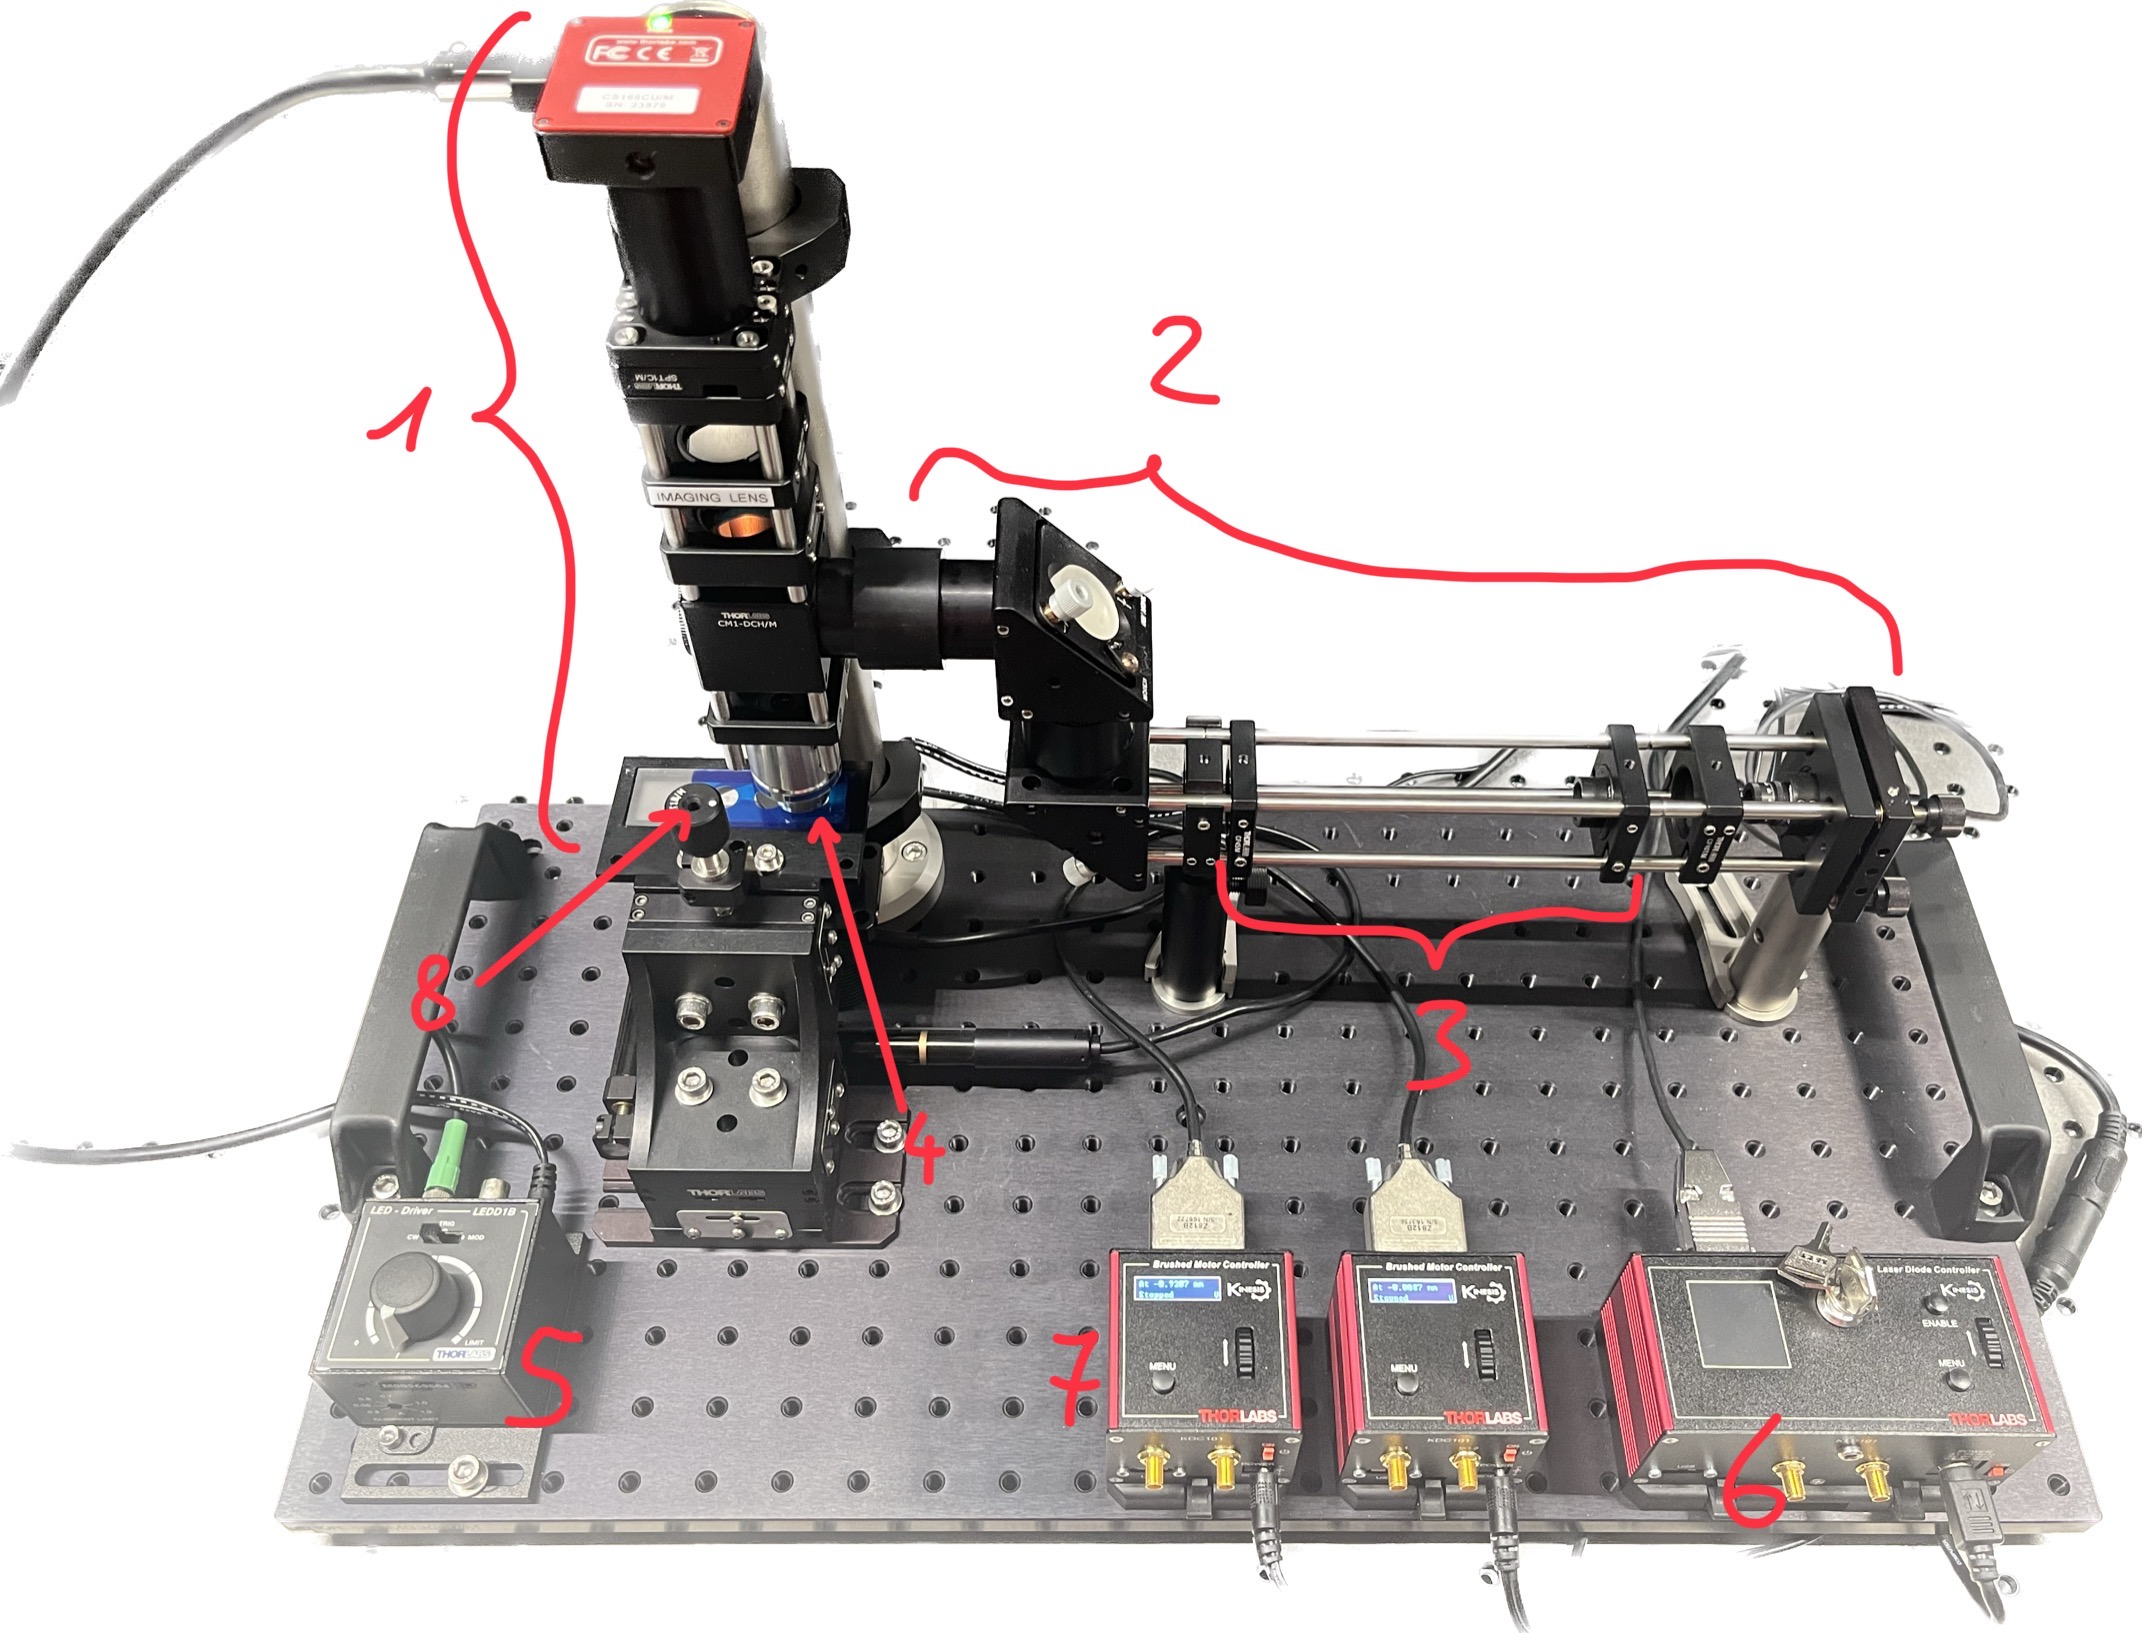
\includegraphics[width =0.7\textwidth]{./figures/aufbau.jpg}
	\end{center}
	\caption[Total experimental setup] { Total experimental setup                                       \\
		1 \dots Microscope module                                      \\
		2 \dots Laser module                                           \\
		3 \dots Telescope module                                       \\
		4 \dots Sample stage                                           \\
		5 \dots Power supply for light                                 \\
		6 \dots Power supply for laser                                 \\
		7 \dots Controller for movement of the sample in x/y-direction \\
		8 \dots Screw for movement of the sample in z-direction
	}\label{fig:aufbau}
\end{figure}

The single optical components, as well as the beampath are visible in
\autoref{fig:aufbau_banzer}.

\begin{figure}[H]
	\begin{center}
		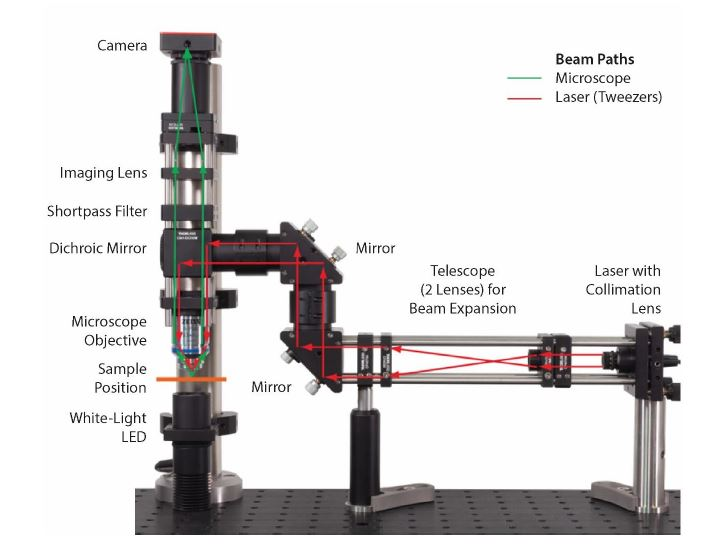
\includegraphics[width =0.9\textwidth]{./figures/aufbau_banzer.JPG}
	\end{center}
	\caption[Optical setup] { Optical setup with drawn beampath
	}\label{fig:aufbau_banzer}%todo \cite{unterlagen}
\end{figure}

\section{Materials}\label{sec:geraeteliste}

For the setup the following parts in \autoref{tab:gerate} are used.

%todo

\begin{table}[H]
	\begin{center}
		\caption{Verwendete Geräte für die Abbildung durch eine Sammellinse
		}
		\begin{tblr}{cells={font=\footnotesize},colspec={lllll}}
			\textbf{Gerätetyp}               & \textbf{Hersteller} & \textbf{Typ} & \textbf{Anmerkung} \\
			Linse                            &                     &              & zu bestimmen       \\
			Lens Mount                       & ThorLabs            & LMR1/M       &                    \\
			Optical Posts                    & ThorLabs            & TR3          &                    \\
			Rail Carrier                     & ThorLabs            & XT34TR1/M    & 3x                 \\
			Halogenlampe                     & ThorLabs            & QTH10/M      &                    \\
			Mount for Rectangular Optics     & ThorLabs            & XYF1/M       &                    \\
			Resolution and Distortion Target & ThorLab             & R1L3S5P      &                    \\
			Aluminium-Schiene                &                     &              &                    \\
			Schirm                           &                     &              & selbst gebaut      \\
			Schibelehre                      & Workzone            & 819547       & digital            \\
		\end{tblr}\label{tab:gerate}
	\end{center}
\end{table}

\section{Implementation and Measurement}\label{sec:versuchsdurchfuehrung_messergebnisse}

\subsection{Microscope}\label{seq:durchfurung_microscope}

For this part only the microscope module form \autoref{fig:aufbau} is needed.

As a sample the Silicas are used. The object holder has a thin placeholder on
it, so that the tiny particles in the liquid are allowed to move, as visible in
\autoref{fig:object_holder}

\begin{figure}[H]
	\begin{center}
		\includegraphics[width =0.5\textwidth]{./figures/Objekt_holde.png}
	\end{center}
	\caption[Object holder with placeholder] { Object holder with placeholder
	}\label{fig:object_holder}
\end{figure}

The object holder is placed on the specimen stage and the camera is connected
with the computer. The analyse of the sample is done with the "ThorCam"\
software. It is important to make sure that there is enough space between the
sample and the detector, to avoid a crash.

Now the white light LED under the sample is switched on in order to create an
image on the software. It is important to keep in mind, that there is a filter
between the sample and the camera to protect it later from the direct incident
of the laser. Thats why the image appears in a greenish shine. Now the sample
is slowly moved upwards in z-direction to create a sharp image.

If the focus is set right, one can observe the brownian motion of the small
particles. Some of them stand still, because the are attached either to the
objective holder or to the cover glass. With the electric controller one can
now navigate over the sample, by selecting an appropriate speed in the menu.

To measure the brownian motion one needs a position on the sample where one
finds at east 3 moving particles at approximately the same size. Then ones
records the screen for at least 2 min to make an analyse of the movement of the
particles. One of these spots is visible in \autoref{fig:pic_brownian_motion},
as an example. The same procedure is again carried out for an other spot.

%todo pic

It is important to keep in mind that after looking at the sample some time it
starts to dry, and gives the particles some kind of a drift towards the middle
of the sample. This can be observed by a "dry-wall" \ that starts to move over
the sample, as visible in \autoref{fig:dry_wall}

% todo pic dry wall

trocknung
\subsection{Lasergun}

For this part of the example the laser module without the telescope is added to
the setup, as visible in \autoref{fig:aufbau}. From now on it is very important
to keep in mind the principles of laser safety and use the laser safety
googles, when the laser is running.

When everything is attached to the setup the laser can be switched on and the
power can slowly be increased.

Now again the z-position of the stage needs to be increased until the focus of
the laser becomes visible in the plane. There are in total 3 positions where
the laser beam is visible which is shown in \autoref{fig:laser_focus}.

%todo pic laserfocus

When the laser is in focus one can try to kick some particles with the laser
beam by varying its power and moving it across the sample.

\subsection{Trapping with laser}

The aim of this experiment is to trap a particle inside the laser beam. This
can be achieved by turning the laser to its highest power witch is at the
explicit case \SI{100}{\milli\ampere} and than bringing it close to a freely
moving particle. The soaking of the particle can be observed. By moving the
laser freely over the sample, the particle can be guided. By varying the power
of the laser one can observe, that an explicit force is needed in order to trap
the particle, depending on its size.

To also increase the power of the laser beam, the telescope cage, visible in
\autoref{fig:aufbau}, is included to the setup, in order to increase the power
of the beam. The interesting thing is, that the telescope had no visible effect
on the trapping of the particle.
%todo sag ma des e oder

Now one particle is trapped and slowly brought to a place on the sample, where
also some other particles of approximately the same size are freely moving, as
visible in \autoref{fig:tapping} and recorded to compare the movement of the
trapped particle with the freely moving one.

%todo trapping

Now one tries to catch 2 particles at the same time. When both particles are
captured by the laser beam and the focus is regulated a bit, by adjusting the
z-position of the sample, the particles can be stacked. In the image it looks
like one particle, but when turning of the laser one can observe both particles
drifting away, as visible in \autoref{fig:stacked}.

%todo fig:stacked

\subsection{Holding force}

The aim of this experiment is to determine the holding force of the laser beam.
Therefore it is important that the focus of the laser is perfectly aligned. To
check this one can try to stack 2 particles, as described before. When the
particles can be stacked, the focus lies in the correct level.

Now one tries to find the speed of the lasermovement, where the particle can
follow. To determine this the speed of the movement can be regulated in the
menu of the controller. In order to find the speed one tries a binary search,
which means always try to divide the interval in 2 sections of approximately
the same size and so look for the speed stepwise. It is important to always try
for the same spot in the sample, because at an other position there could be
other conditions and so the results can not be compared. It is also important
to keep in mind the drift due to the dry of the sample, as already mentioned in
\autoref{seq:durchfurung_microscope}. This procedure is now repeated for
different laser powers and for 2 different particle sizes. The results are
visible in \autoref{tab:movement}.

%todo tab movement

\subsection{Characterization of unknown sample}

For this part the sample is changed. When removing the object holder vit is
important to go down in z-direction with the sample stage in order to do not
hit the objective by changing the sample.

Now the objective colder can be cleaned and the new sample, labeled "unknown"\
placed on it.

When everything is attached and the laser beam is in focus again, one can try
to search new particles. What one immediately sees is, that the new sample
seems to contain particles that can absorb the laser beam, because one cam
"blow" \ them up.

%todo foto

What one can also observe with the bare eye is that the whole sample seems red
although there are also e few particles inside it, so the have a huge coloring
effect.

\subsection{Trapping of living organisms}

For this part of the experiment one needs a sample with living bacteria on it.
Therefore a gulp of "ayran" \ gets diluted with water to make it transparent.

When everything is aligned and the laser is switched on again, one can try to
find a bacterium. The can be easily detected due to the movement. When one
traps the particle with the laser beam one can immediately observe, that it
stops its movement and aligns with the laser beam, as visible in
\autoref{fig:bacterium}.

%todo bacterium

\subsection{Transfer of angular momentum}

For this part of the experiment the sample "vaterite" \ is used. To avoid
pollution of the "ayran"\ sample this sample is placed on a new object holder.

When everything is aligned one navigates through the sample and searches for a
particle that looks round but has a slight discontinuity, to later observe
rotations of it.

To transfer the angular momentum of the laser one has to change its handyness.
This is done by holding a waveplate into the telescope and rotating it while
observing the trapped particle.

Unfortunately the rotational effect was not as strong as expected. This can be
explained, because many parameters need to fit in order to create that effect.

%todo willst du da no mehr schreiben dazu?

\section{Analysis}\label{sec:auswertung}

Um zu sehen wie sich die Unsicherheit der Messungen bis in die Ergebnisse
fortpflanzt, ist erweiterte Gauss-Methode verwendet worden. Die Grundlagen
dieser Methode stammen von den Powerpointfolien von
% GUM~\cite{wolfgang_kessel_isobipm-gum_2004}. Für die Auswertung ist die
Progammiersprache Python im speziellen die Pakete \verb#labtool-ex2#,
\verb#pandas#, \verb#sympy#, \verb#lmfit# zur Hilfe genommen worden.
\verb#lmfit# wurde für das Fitten verwendet, \verb#sympy# wurde für symbolische
Manipulation verwendet und die restlichen Pakete für leichteres Handhaben der
Daten. Dies wurde aber alles durch \verb#labtool-ex2# abstrahiert.

Um höchstmögliche Genauigkeit zu garantieren wird erst bei der Darstellung der
Wert in Tabellen gerundet.

\subsection{Microscope}

\begin{figure}[H]
	\centering
	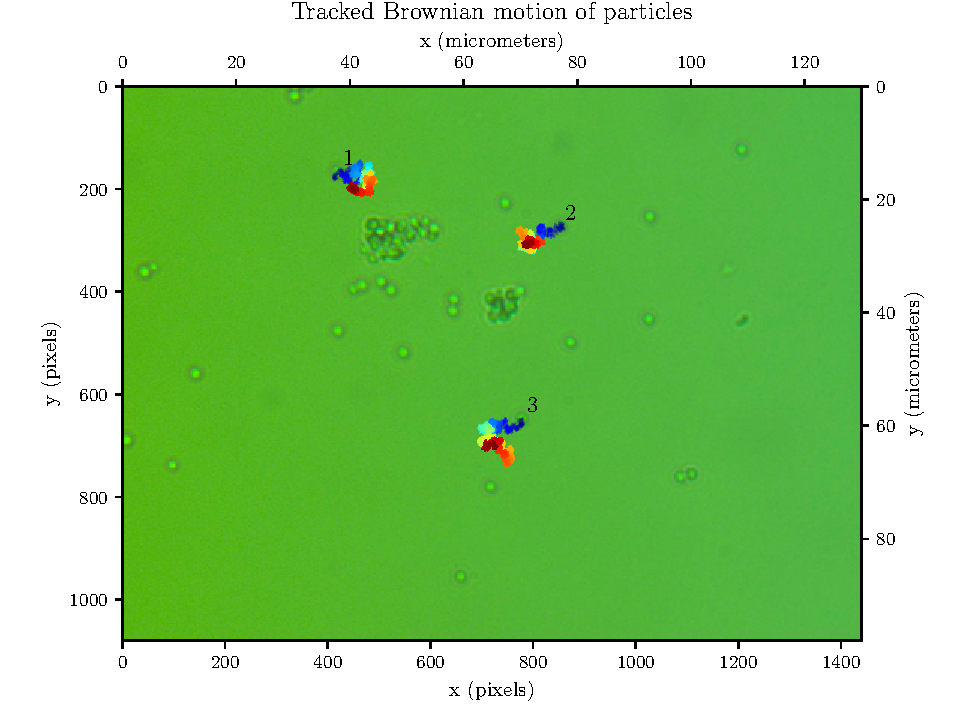
\includegraphics[width=0.95\textwidth]{figures/I1_tracked.pdf}
	\caption[Capture 1 of particles]{This figure contains the initial conditions of the
		tracked region displayed in the background and has the trajectories of the
		particles overlaid from cold to hot indicating the time evolution of the
		particles. Furthermore, the particles are labeled and plotted on an x, y
		coordinate grid. This is the first capture of
		particles.
	}\label{fig:part_overview_1}
\end{figure}

\begin{figure}[H]
	\centering
	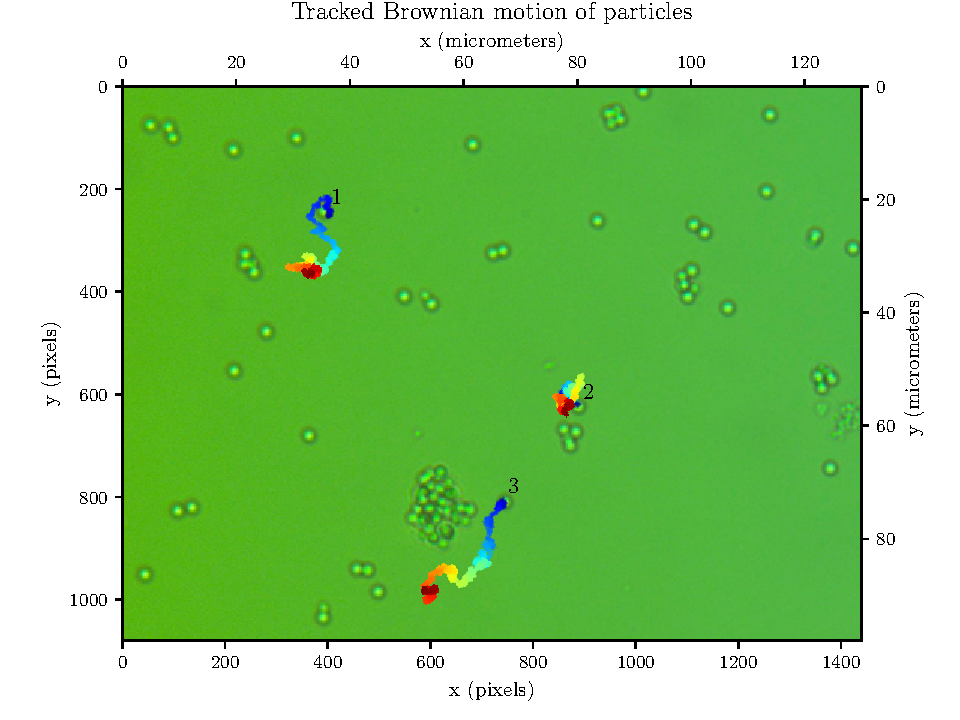
\includegraphics[width=0.95\textwidth]{figures/I2_tracked.pdf}
	\caption[Capture 2 of particles]{This figure contains the initial conditions of the
		tracked region displayed in the background and has the trajectories of the
		particles overlaid from cold to hot indicating the time evolution of the
		particles. Furthermore, the particles are labeled and plotted on an x, y
		coordinate grid. This is the second capture of
		particles.
	}\label{fig:part_overview_2}
\end{figure}

\begin{figure}[H]
	\centering
	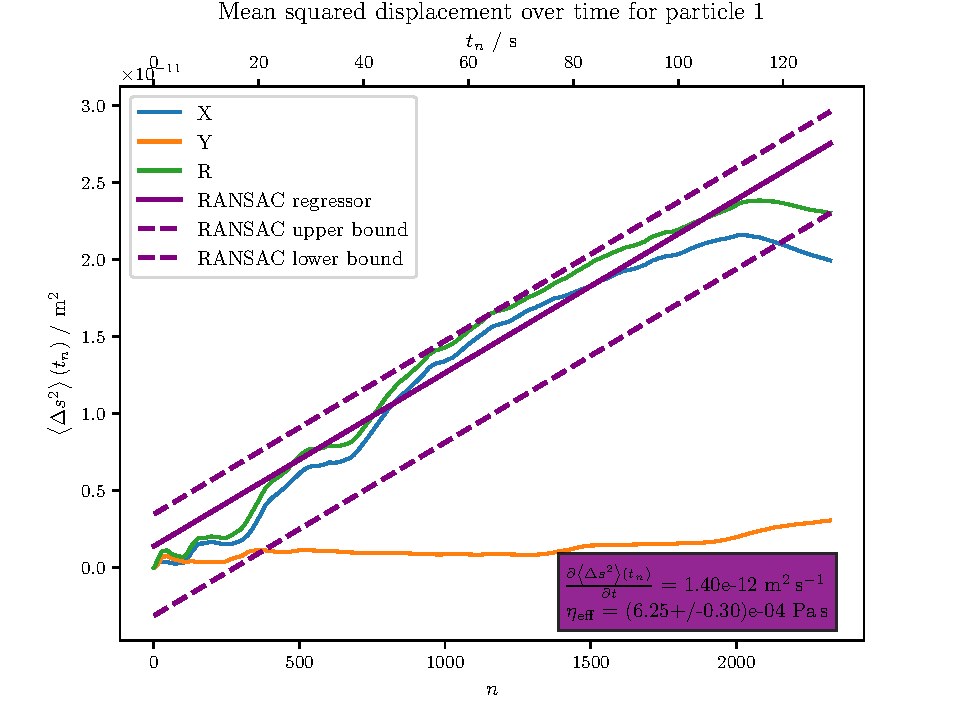
\includegraphics[width=0.48\textwidth]{figures/I1_particle_1.pdf}
	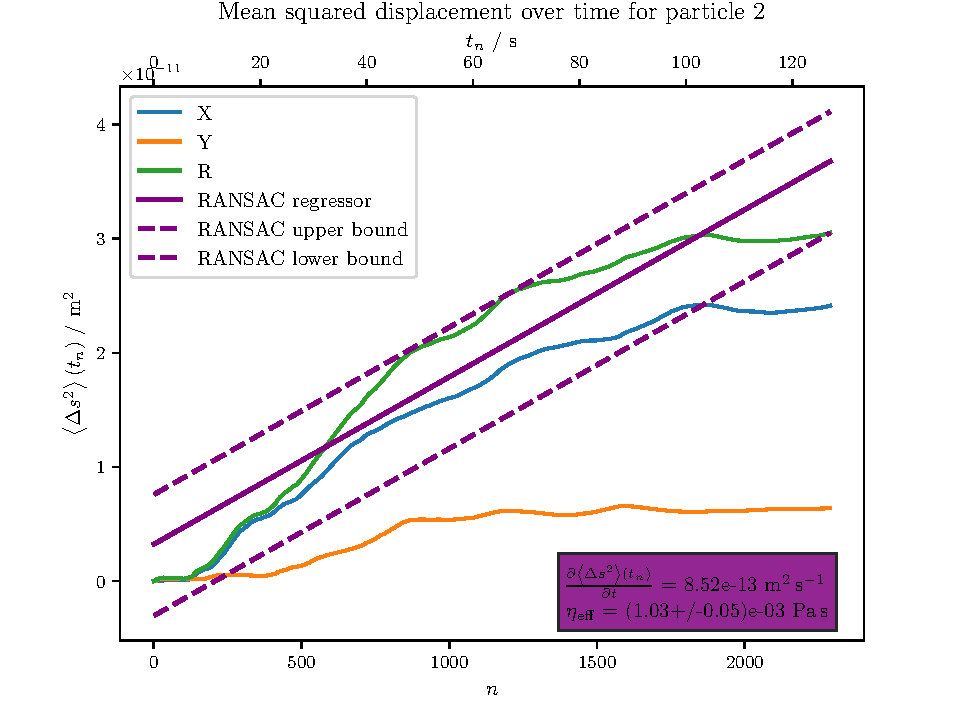
\includegraphics[width=0.48\textwidth]{figures/I1_particle_2.pdf}
	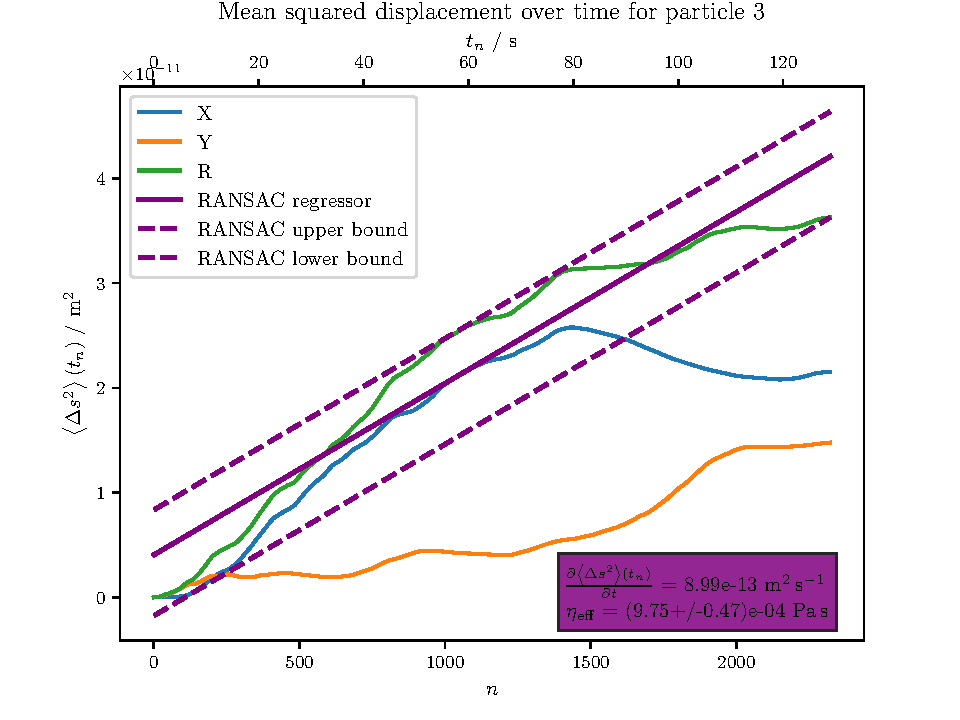
\includegraphics[width=0.48\textwidth]{figures/I1_particle_3.pdf}
	\caption[Time averaged mean squared displacements from the particles of the first
		capture]{This figure one can see the time averaged mean squared displacements
		($\left\langle \Delta s^2 \right\rangle(t_n)$) (averaged up to every time step
		$t_n$) in X and Y direction and the radial direction R. The labels correspond
		to particles in \autoref{fig:part_overview_1}.
	}\label{fig:part_first}
\end{figure}

\begin{figure}[H]
	\centering
	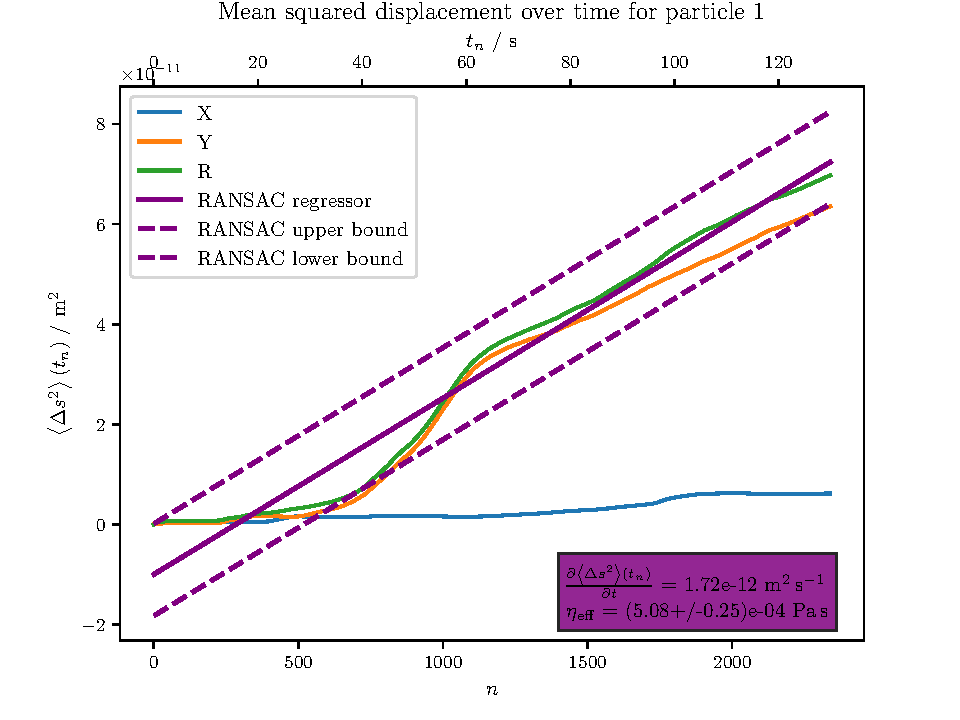
\includegraphics[width=0.48\textwidth]{figures/I2_particle_1.pdf}
	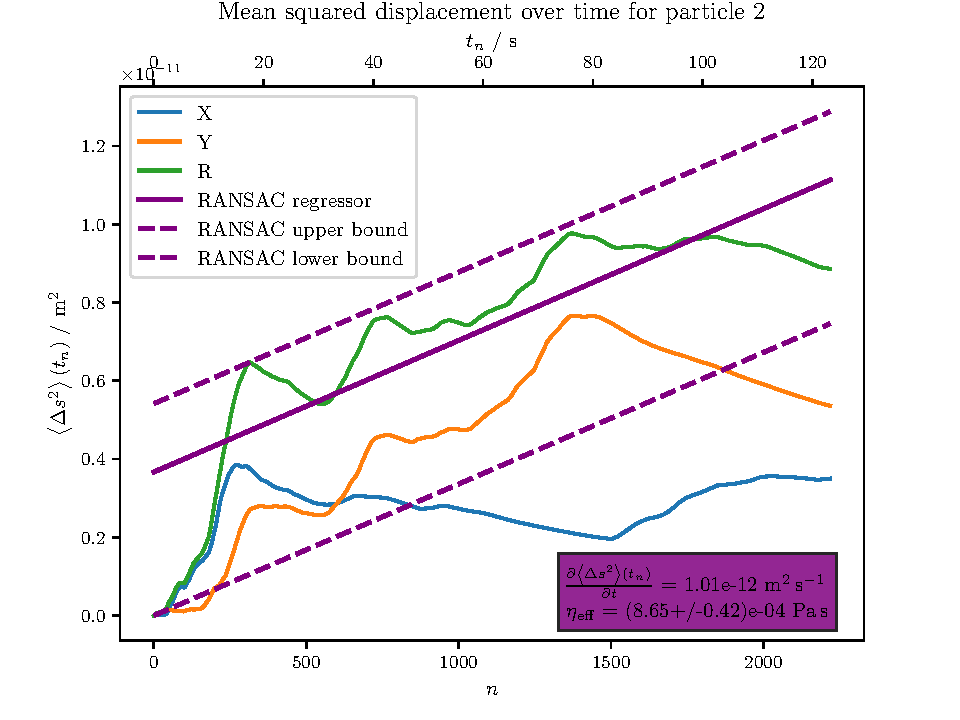
\includegraphics[width=0.48\textwidth]{figures/I2_particle_2.pdf}
	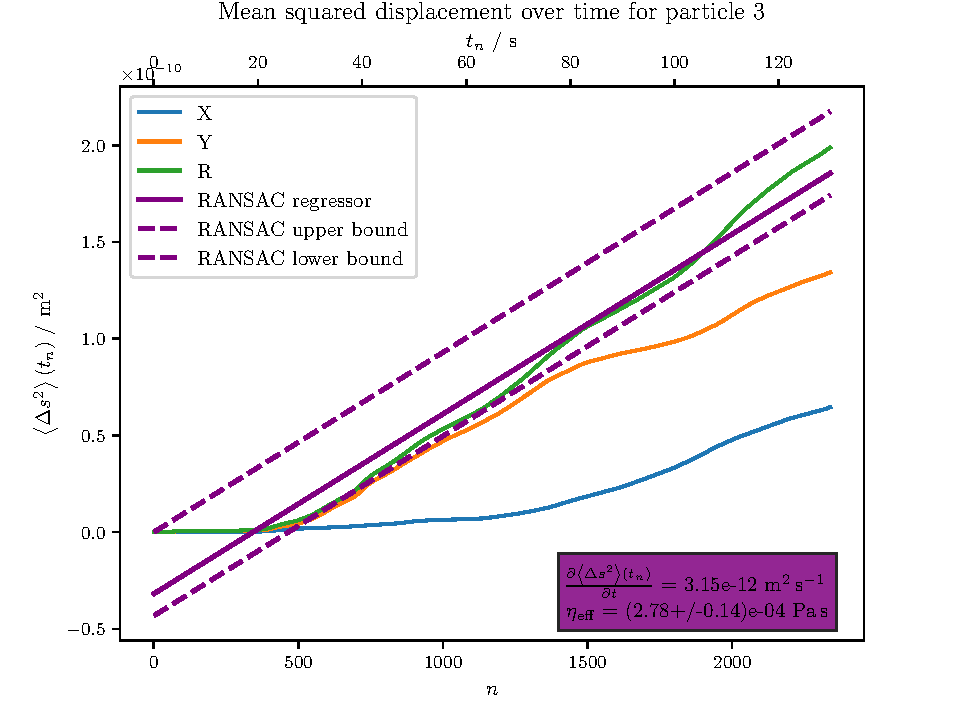
\includegraphics[width=0.48\textwidth]{figures/I2_particle_3.pdf}
	\caption[Time averaged mean squared displacements from the particles of the second
		capture]{This figure one can see the time averaged mean squared displacements
		($\left\langle \Delta s^2 \right\rangle(t_n)$) (averaged up to every time step
		$t_n$) in X and Y direction and the radial direction R. The labels correspond
		to particles in \autoref{fig:part_overview_2}.
	}\label{fig:part_second}
\end{figure}

\subsection{Lasergun}

\subsection{Trapping with laser}

\begin{figure}[H]
	\centering
	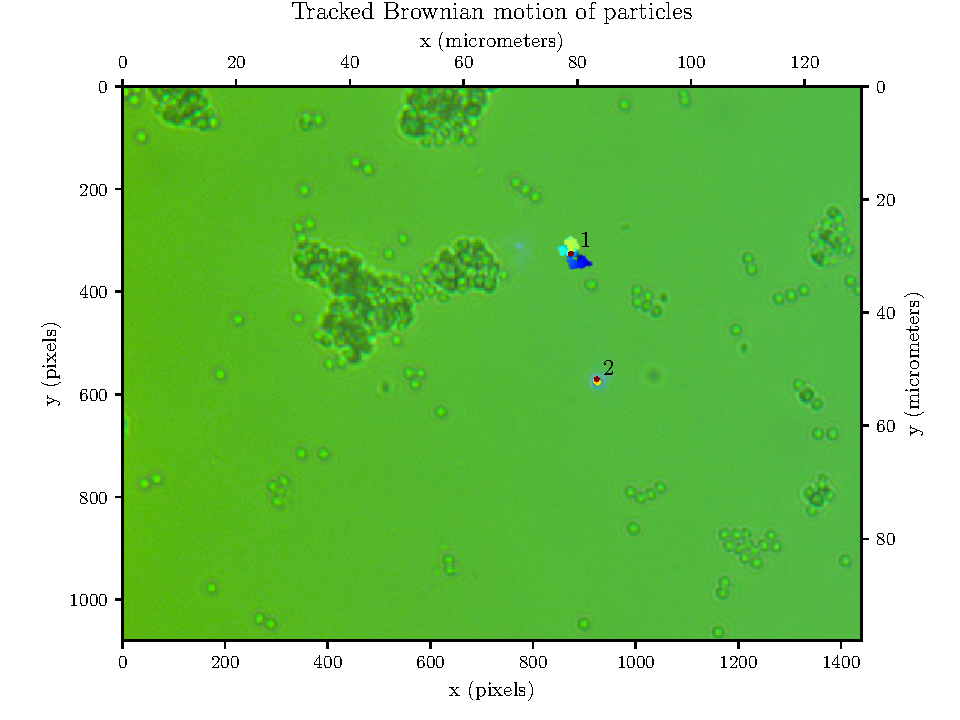
\includegraphics[width=0.95\textwidth]{figures/III_tracked.pdf}
	\caption[Capture of trapped particle]{This figure contains the initial conditions of the
		tracked region displayed in the background and has the trajectories of the
		particles overlaid from cold to hot indicating the time evolution of the
		particles. Furthermore, the particles are labeled and plotted on an x, y
		coordinate grid. This tracking captured two particles first particle (1) is
		free and the second particle (2) is trapped.
	}\label{fig:part_overview_trap}
\end{figure}

\begin{figure}[H]
	\centering
	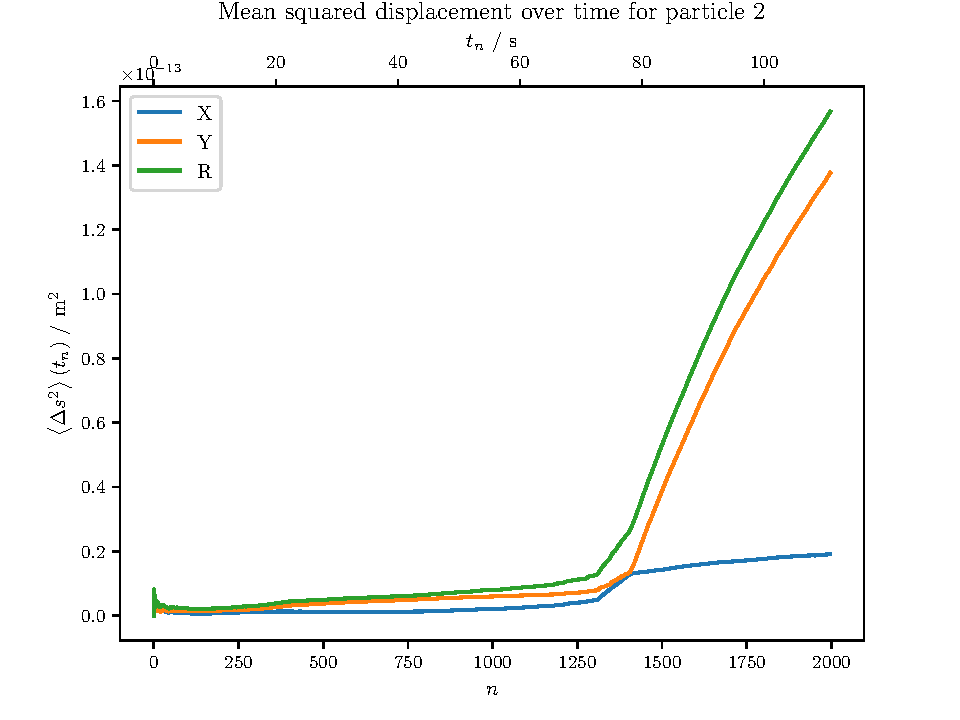
\includegraphics[width=0.95\textwidth]{figures/III_particle_trapped.pdf}
	\caption[Time averaged mean squared displacements of trapped particle]{This figure one
		can see the time averaged mean squared displacements ($\left\langle \Delta s^2
			\right\rangle(t_n)$) (averaged up to every time step $t_n$) in X and Y
		direction and the radial direction R for the trapped particle. The labels
		correspond to particles in \autoref{fig:part_overview_trap}. Furthermore, the
		trapping was turned off at around step $n=1250$ to contrast trapped vs free.
	}\label{fig:part_trapped}
\end{figure}

\begin{equation}
	\eta_\text{eff} = \frac{2k_B T}{3\pi s R}
	\label{eq:eff_visc}
\end{equation}

Using the slope of the fitted lines $s$, the radius of the spherical particles
$R=\SI{2.06}{\micro\meter}$ and the medium temperature of
$T=\SI{308.15(15.00)}{\kelvin} = \SI{35(15)}{\celsius}$ we can calculate the
effective viscosity $\eta_\text{eff}$. Here the temperature was assumed to be
the \SI{20}{\celsius} above the room temperature. Since the irradiance of lamp
was heating up the liquid. This is the only uncertainty considered in the
calculation of $\eta_\text{eff}$. Since the RANSAC-Regressor was used to find
the slopes and this method of fitting does not provide uncertainties for the
fitted parameters. It would be possible to calculate the uncertainty of the
slope by using the least squares method for fitting after removing the
outliers. But this was not done in this case, since we use the obtained
effective viscosities to derive a representative effective viscosity using the
median statistic (for its robustness against outliers) is used for the $\mu$
estimator. This is allowed if the underling distribution is symmetric and with
finite mean has a median equal to its mean. This is the case if this estimator
will vary like a normal distribution and thus the error will be calculated
using the standard mean error.

\begin{table}[H]
	\caption[Collected effective viscosities]{This table contains the effective viscosities
		$\eta_\text{eff}$ of all the tracked particles from \autoref{fig:part_first}
		and \autoref{fig:part_second}, which where calculated using
		\autoref{eq:eff_visc}. Here is only the uncertainty due to actual temperature
		in the fluid considered in the measured effective viscosities. Using the median
		statistic and the standard mean error the estimator for the true
		$\hat{\eta_\text{eff}}$ is calculated.
	}\label{tab:eff_visc} \centering
	\begin{tblr}{colspec={lc}}
		                                             & $\eta_\text{eff}$                    \\
		Capture 1 Particle 1                         & \SI{0.63(30) }{\milli\pascal\second} \\
		Capture 1 Particle 2                         & \SI{1.03(5) }{\milli\pascal\second}  \\
		Capture 1 Particle 3                         & \SI{0.97(5) }{\milli\pascal\second}  \\
		Capture 2 Particle 1                         & \SI{0.51(3) }{\milli\pascal\second}  \\
		Capture 2 Particle 2                         & \SI{0.87(4) }{\milli\pascal\second}  \\
		Capture 2 Particle 3                         & \SI{0.278(14)}{\milli\pascal\second} \\
		$\hat{\theta}(\mu(\eta_\text{eff}))$         & \SI{0.87}{\milli\pascal\second}      \\
		SEM($\eta_\text{eff}$)                       & \SI{0.267}{\milli\pascal\second}     \\
		$\Delta\eta_{\text{eff}_\text{Temperature}}$ & \SI{0.04}{\milli\pascal\second}      \\
		$\hat{\eta_\text{eff}}$                      & \SI{0.9(4)}{\milli\pascal\second}
	\end{tblr}
\end{table}

\subsection{Holding force}

\begin{table}
	\caption{This table contains measured velocities and whether the particle
		remained trapped moving with the velocity at a certain laser power.
		All velocities are measured in \si{\milli\meter\per\second}. Here
		is max power of the laser diode \SI{50}{\milli\watt} at \SI{100}{\milli\ampere}
		driver current. In the last row the chosen velocities for their respective
		categories are displayed. In the \SI{50}{\percent} category the results
		were averaged and in the \SI{100}{\percent} category the last binding
		velocity was used. The uncertainties are due the discretization of the actuator velocity,
		and the uncertainty are for all the velocities is $\SI{0.002}{\milli\meter\per\second}$.
	}\label{tab:velocities}
	\centering
	\begin{tblr}{colspec={cc|cc|cc|cc}}
		\SetCell[c=4]{c} $@\SI{50}{\percent}$ Power   &          &                                &          & \SetCell[c=4]{c} $@\SI{100}{\percent}$ Power &          &                                 &          \\
		$v_\text{Big} / \si{\milli\meter\per\second}$ & Trapped? & $v_\text{Small}$               & Trapped? & $v_\text{Big}$                               & Trapped? & $v_\text{Small}$                & Trapped? \\
		\num{0.081}                                   & \bot     & \num{0.071}                    & \bot     & \num{0.250}                                  & \bot     & \num{0.087}                     & \bot     \\
		\num{0.051}                                   & \bot     & \num{0.035}                    & \bot     & \num{0.106}                                  & \bot     & \num{0.071}                     & \bot     \\
		\num{0.044}                                   & \bot     & \num{0.021}                    & \bot     & \num{0.094}                                  & \bot     & \num{0.062}                     & \top     \\
		\num{0.030}                                   & \bot     & \num{0.018}                    & \bot     & \num{0.080}                                  & \sim     &                                 &          \\
		\num{0.025}                                   & \bot     & \num{0.016}                    & \bot     & \num{0.076}                                  & \sim     &                                 &          \\
		\num{0.023}                                   & \top     & \num{0.014}                    & \top     & \num{0.062}                                  & \top     &                                 &          \\
		\num{0.021}                                   & \top     & \num{0.011}                    & \top     & \num{0.053}                                  & \top     &                                 &          \\
		\num{0.018}                                   & \top     & \num{0.005}                    & \top     & \num{0.030}                                  & \top     &                                 &          \\ \hline
		\SetCell[c=2]{c}\num{0.024(2)}                &          & \SetCell[c=2]{c}\num{0.015(2)} &          & \SetCell[c=2]{c}\num{0.062(2)}               &          & \SetCell[c=2]{c} \num{0.062(2)} &
	\end{tblr}
\end{table}

\begin{equation}
	\vert F_\text{trap} \vert =\vert k \delta x \vert = F_\text{Stoke}  = 6 \pi R \eta_\text{eff} v
	\label{eq:holding_force}
\end{equation}

\begin{table}
	\caption{This table contains the calculated holding forces $F_\text{trap}$ using \autoref{eq:holding_force}
		and the obtained value for the effective viscosity $\eta_\text{eff}$ from \autoref{tab:eff_visc} and the
		values for the critical holding velocities from \autoref{tab:velocities}.
	}\label{tab:holding_forces}
	\centering
	\begin{tblr}{colspec={lc}}
		                          & $F_\text{trap}$             \\
		Big @\SI{50}{\percent}    & \SI{0.43(16)}{\pico\newton} \\
		Big @\SI{100}{\percent}   & \SI{1.1(4)}{\pico\newton}   \\
		Small @\SI{50}{\percent}  & \SI{0.19(8)}{\pico\newton}  \\
		Small @\SI{100}{\percent} & \SI{0.8(3)}{\pico\newton}
	\end{tblr}
\end{table}

% probably we are in the second focus not the third which means that the particles are pulled to the 
% glass interface. This would explain a reduced holding force due to scraping and that the effective 
% viscosity conforms to the literature value. Furthermore this would
% also explain the why the angular momentum transfer didn't work.

\subsection{Characterization of unknown sample}

\subsection{Trapping of living organisms}

\subsection{Transfer of angular momentum}

\section{Diskussion}\label{sec:diskussion}

\subsection{Microscope}

\subsection{Lasergun}

\subsection{Trapping with laser}

\subsection{Holding force}

\subsection{Characterization of unknown sample}

\subsection{Trapping of living organisms}

\subsection{Transfer of angular momentum}

\section{Zusammenfassung}\label{sec:zusammenfassung}

\subsection{Microscope}

\subsection{Lasergun}

\subsection{Trapping with laser}

\subsection{Holding force}

\subsection{Characterization of unknown sample}

\subsection{Trapping of living organisms}

\subsection{Transfer of angular momentum}

\newpage
\printbibliography
%todo literatur
\listoffigures
\listoftables
\end{document}
